\section{Gitting started}	% huehue

\subsection{Repository aanmaken}
\begin{frame}[fragile]
	%\frametitle{Repository aanmaken}
	\begin{enumerate}
		\item Open terminal (windows: \alert{git-bash})
		\item \texttt{cd} naar map die je wil bijhouden
			(of \texttt{mkdir} een nieuwe)
		\item \texttt{git init}
		\item \texttt{git status}
	\end{enumerate}
	Als het goed is zie je nu \alert{niet}:
	\begin{minted}{text}
fatal: Not a git repository or 
	any of the parent directories: .git
	\end{minted}
\end{frame}

\subsection{Bestanden laten bijhouden}
\begin{frame}[fragile]
	\begin{enumerate}
		\item \texttt{git status}
		\item Bekijk 'untracked files'
		\item \texttt{git add bestand1 bestand2 map1}\\ of:
			\texttt{git add .}\\
			(map pakt alle bestanden erin mee, . is huidige map)
		\item \texttt{git commit -m "Eerste commit"}
	\end{enumerate}
	Resultaat: 
	\begin{minted}{text}
	[master 1234abc] Eerste commit
	x files added
	\end{minted}
\end{frame}

\frame{
	\begin{center}
		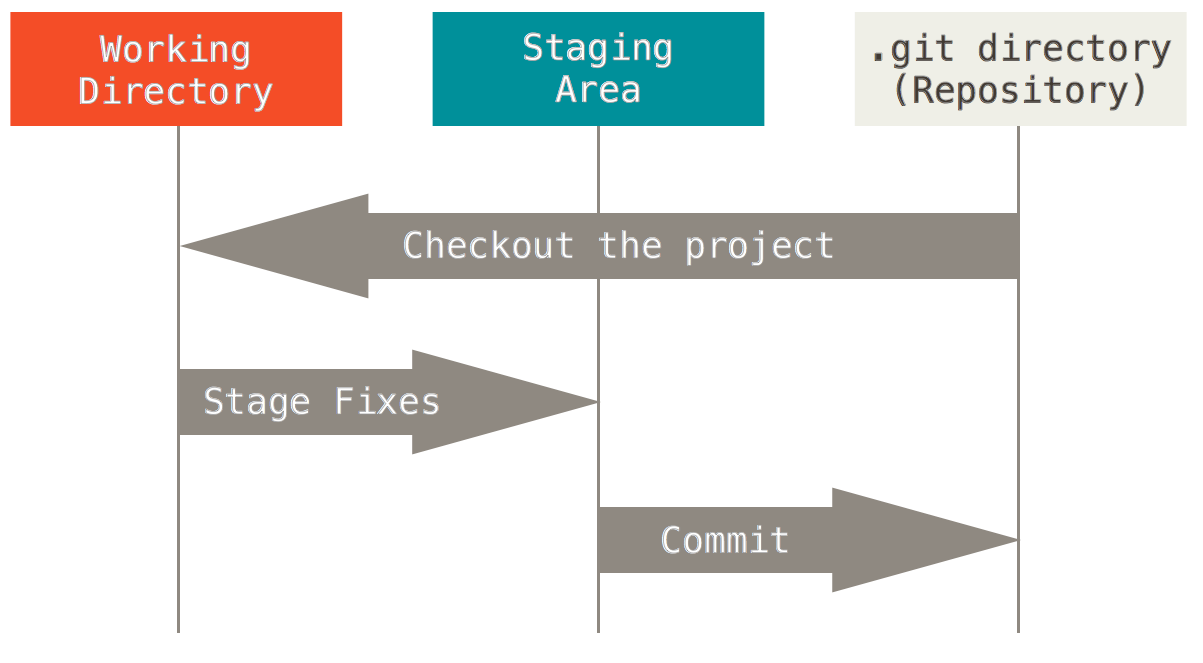
\includegraphics[width=\textwidth]{images/areas}
	\end{center}
	\begin{itemize}
		\item \texttt{git add} $\rightarrow$ 'Stage Fixes'
		\item \texttt{git commit} $\rightarrow$ 'Commit'
	\end{itemize}
}
